\hypertarget{interfaceCqrs_1_1Commands_1_1ICommandHandler}{}\section{Cqrs.\+Commands.\+I\+Command\+Handler$<$ T\+Authentication\+Token, in in T\+Command $>$ Interface Template Reference}
\label{interfaceCqrs_1_1Commands_1_1ICommandHandler}\index{Cqrs.\+Commands.\+I\+Command\+Handler$<$ T\+Authentication\+Token, in in T\+Command $>$@{Cqrs.\+Commands.\+I\+Command\+Handler$<$ T\+Authentication\+Token, in in T\+Command $>$}}


An I\+Command\+Handler$<$\+T\+Authentication\+Token,\+T\+Command$>$ receives an I\+Command$<$\+T\+Authentication\+Token$>$ and brokers a result from the appropriate I\+Aggregate\+Root$<$\+T\+Authentication\+Token$>$. \char`\"{}\+A result\char`\"{} is either a successful application of the command, or an exception. This is the common sequence of steps an I\+Command\+Handler$<$\+T\+Authentication\+Token,\+T\+Command$>$ might follow\+:  


Inheritance diagram for Cqrs.\+Commands.\+I\+Command\+Handler$<$ T\+Authentication\+Token, in in T\+Command $>$\+:\begin{figure}[H]
\begin{center}
\leavevmode
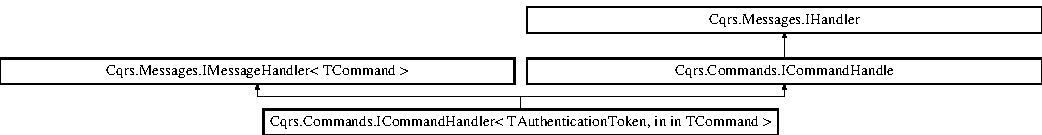
\includegraphics[height=1.810345cm]{interfaceCqrs_1_1Commands_1_1ICommandHandler}
\end{center}
\end{figure}
\subsection*{Additional Inherited Members}


\subsection{Detailed Description}
An I\+Command\+Handler$<$\+T\+Authentication\+Token,\+T\+Command$>$ receives an I\+Command$<$\+T\+Authentication\+Token$>$ and brokers a result from the appropriate I\+Aggregate\+Root$<$\+T\+Authentication\+Token$>$. \char`\"{}\+A result\char`\"{} is either a successful application of the command, or an exception. This is the common sequence of steps an I\+Command\+Handler$<$\+T\+Authentication\+Token,\+T\+Command$>$ might follow\+: 

Validate the I\+Command$<$\+T\+Authentication\+Token$>$ on its own merits. Ask an I\+Aggregate\+Root$<$\+T\+Authentication\+Token$>$ to handle the I\+Command$<$\+T\+Authentication\+Token$>$. If validation is successful, 0..n I\+Event$<$\+T\+Authentication\+Token$>$ artefacts (1 is common) are queued for publishing. Attempt to persist the new I\+Event$<$\+T\+Authentication\+Token$>$ artefacts. If there\textquotesingle{}s a concurrency conflict during this step, either give up, or retry things. Dispatch the queued I\+Event$<$\+T\+Authentication\+Token$>$ artefacts. 

Should a I\+Command\+Handler$<$\+T\+Authentication\+Token,\+T\+Command$>$ affect one or several I\+Aggregate\+Root$<$\+T\+Authentication\+Token$>$s?

Only one.

Do I put logic in I\+Command\+Handler$<$\+T\+Authentication\+Token,\+T\+Command$>$?

Yes. Exactly what logic depends on your factoring. The logic for validating the I\+Command$<$\+T\+Authentication\+Token$>$ on its own merits always gets executed in the I\+Command\+Handler$<$\+T\+Authentication\+Token,\+T\+Command$>$, although we recommend refactoring these into an I\+Command\+Validator$<$\+T\+Authentication\+Token,\+T\+Command$>$. Provided validation is successful we recommend a more functional factoring, where the I\+Aggregate\+Root$<$\+T\+Authentication\+Token$>$ exists independently of the I\+Command\+Handler$<$\+T\+Authentication\+Token,\+T\+Command$>$ and the next step would be to load the I\+Aggregate\+Root$<$\+T\+Authentication\+Token$>$ from the I\+Unit\+Of\+Work$<$\+T\+Authentication\+Token$>$ and request the I\+Aggregate\+Root$<$\+T\+Authentication\+Token$>$ handle the I\+Command$<$\+T\+Authentication\+Token$>$ itself. The I\+Unit\+Of\+Work$<$\+T\+Authentication\+Token$>$ should then have uncommitted I\+Event$<$\+T\+Authentication\+Token$>$ artefacts as a results of asking the I\+Aggregate\+Root$<$\+T\+Authentication\+Token$>$ to handle the I\+Command$<$\+T\+Authentication\+Token$>$. Finally the I\+Command\+Handler$<$\+T\+Authentication\+Token,\+T\+Command$>$ should instruct the I\+Unit\+Of\+Work$<$\+T\+Authentication\+Token$>$ to I\+Unit\+Of\+Work$<$\+T\+Authentication\+Token$>$.\+Commit all uncommited I\+Event$<$\+T\+Authentication\+Token$>$ artefacts.

However you have it, the logic boils down to validation and some sequence of steps that lead to the I\+Command$<$\+T\+Authentication\+Token$>$ becoming an Exception or I\+Event$<$\+T\+Authentication\+Token$>$(s). If you\textquotesingle{}re tempted to go beyond this, see the rest of the remarks.

Can I call a read side (such as a read store, data store or I\+Repository$<$\+T\+Authentication\+Token$>$) from my I\+Command\+Handler$<$\+T\+Authentication\+Token,\+T\+Command$>$?

No.

Can I do logging, security, or auditing in my I\+Command\+Handler$<$\+T\+Authentication\+Token,\+T\+Command$>$?

Yes. The decorator pattern comes in handy here to separate those concerns neatly.

How are conflicts between concurrent I\+Command$<$\+T\+Authentication\+Token$>$s handled in the I\+Command\+Handler$<$\+T\+Authentication\+Token,\+T\+Command$>$?

The place where the new I\+Event$<$\+T\+Authentication\+Token$>$ artefacts for the I\+Aggregate\+Root$<$\+T\+Authentication\+Token$>$ are persisted is the only place in the system where we need to worry about concurrency conflicts. The I\+Event\+Store$<$\+T\+Authentication\+Token$>$ knows the sequence number of the latest I\+Event$<$\+T\+Authentication\+Token$>$ applied on that I\+Aggregate\+Root$<$\+T\+Authentication\+Token$>$, and the I\+Command\+Handler$<$\+T\+Authentication\+Token,\+T\+Command$>$ knows the sequence number of the last I\+Event$<$\+T\+Authentication\+Token$>$ it read. If these numbers do not agree, it means some other thread or process got there first. The I\+Command\+Handler$<$\+T\+Authentication\+Token,\+T\+Command$>$ can then load up the events again and make a new attempt.

Should I do things that have side-\/effects in the outside world (such as sending email) directly in a I\+Command\+Handler$<$\+T\+Authentication\+Token,\+T\+Command$>$?

No, since a concurrency conflict will mean the I\+Command\+Handler$<$\+T\+Authentication\+Token,\+T\+Command$>$ logic will be run again. Do such things in an Apply I\+Event$<$\+T\+Authentication\+Token$>$ method in an I\+Aggregate\+Root$<$\+T\+Authentication\+Token$>$. 

 Also see \href{http://cqrs.nu/Faq/command-handlers}{\tt http\+://cqrs.\+nu/\+Faq/command-\/handlers}. \begin{Desc}
\item[Type Constraints]\begin{description}
\item[{\em T\+Command} : {\em \hyperlink{interfaceCqrs_1_1Commands_1_1ICommand}{I\+Command}$<$T\+Authentication\+Token$>$}]\end{description}
\end{Desc}
